% !TEX root=main.tex

To design approximations, it will be useful to view Equation \ref{eqn:argmax-path} as a graph optimisation problem
for the case of structured SVMs with pairwise potentials.
Here, the score $f(\mathbf{x}, \mathbf{y})$ can be decomposed as
%$$ f(\mathbf{x}, \mathbf{y}) = \sum_{k = 1}^{|\mathbf{y}|} \mathbf{w}_k^T \Phi( \mathbf{x}, y_k ) + \sum_{j, k = 1}^{|\mathbf{y}|} \mathbf{w}_{j k}^T \Phi( \mathbf{x}, y_k, y_j ) $$
%for unary and pairwise weight vectors $\mathbf{w}_k$.
\begin{equation}
	\label{eqn:f-ssvm}
	f(\mathbf{x}, \mathbf{y}) = \sum_{k = 1}^{|\mathbf{y}|} \alpha( y_k ) + \sum_{k = 1}^{|\mathbf{y}| - 1} \beta( y_k, y_{k+1} )
\end{equation}
for suitable unary and pairwise potentials $\alpha, \beta$~\cite{Chen:2017}.
Consider then a complete graph where the nodes are POIs, each node $p \in \PCal$ has a score $\alpha( p )$, and each edge $(p, p') \in \PCal^2$ has a score $\beta( p, p' )$.
Then, Equation \ref{eqn:argmax-path} is equivalently a problem of selecting $l$ nodes whose
total sum of node and edge scores maximises Equation \ref{eqn:f-ssvm}.
% This points to a natural means of approximation: solve this selection problem greedily, or fix the set of nodes and only solve the ordering problem.
%the following selection problem:
%$$	r( x ) = \argmax_{\mathbf{y} \in \thickbar{\YCal}_x}~\sum_{k = 1}^{|\mathbf{y}|} \alpha( y_k ) + \sum_{j, k = 1}^{|\mathbf{y}|} \beta( y_k, y_j ). $$
We now look at ways of approximately solving this selection problem.

\subsection{Heuristic loop elimination}
\label{sec:loop-elim}
% !TEX root=main.tex

%An even simpler approach than the above greedy strategy is the following:
Perhaps the simplest approximate solution to Equation \ref{eqn:argmax-path} is to simply remove the first loop occurring in the standard Viterbi solution (Equation \ref{eqn:argmax}).
Specifically, if the Viterbi solution is $( y_1, \ldots, y_l )$,
and $i$ is the first index where $y_i$ already appears in the subsequence $( y_1, \ldots, y_{i-1} )$,
then simply return the subsequence $( y_1, \ldots, y_{i-1} )$.

From a graph perspective, this approach makes the directed sub-graph induced by the Viterbi solution acyclic
by simply breaking the first cycle-inducing edge.
This is sensible if sequences never escape the first cycle, \ie after the first repeated POI, there is no new POI.
We have indeed found this to be the case in our problem (perhaps owing to cycles being induced by dominant edge scores).
More generally, for sequences %such as $(1,2,1,3)$
where there is a repeated POI followed by a new POI,
the problem of removing cycles can be seen as a special case of the ({\sf NP}-hard) minimum feedback arc-set problem.

This algorithm is appealing in its simplicity,
but has at least two detrimental features.
First, it makes the questionable assumption that we can solve Equation \ref{eqn:argmax-path} from the standard Viterbi solution alone.
Second, it returns a solution that violates the length constraint of the path recommendation problem.
As a remedy to this, we can request the Viterbi algorithm to return a path of longer length $l' > l$;
of course, there is no clear means of choosing $l'$ so that the result is exactly of length $l$.

% Second, if we restrict attention to the POIs $\{ y_1, \ldots, y_{i-1} \}$, it is unclear whether the original ordering of the subsequence is optimal.
% The second point can be remedied, as we now see.


\subsection{Greedy path discovery}
\label{sec:greedy}
% !TEX root=main.tex

In light of the graph-based view, a natural approach to approximately solve Equation \ref{eqn:argmax-path} is a greedy algorithm.
Suppose we have already determined a partial path comprising distinct POIs $y_1, \ldots, y_k$.
Then, we can select the next candidate POI $y_{k + 1}$ as
the node
that iteratively optimises Equation \ref{eqn:f-ssvm},
%whose combined node- and edge-score is maximum,
subject to the constraint that it is distinct from all other nodes in the current path;
formally, we pick
%the node whose combined node score $\alpha( y_{k + 1} )$ and
%transition score $\beta( y_{k}, y_{k + 1} )$
$$ y_{k + 1} = \argmax_{p \in \PCal - \{ y_1, \ldots, y_k \}} \alpha( p ) + \beta( y_k, p ). $$
This algorithm is faster than the above heuristic, with $\mathscr{O}(l \cdot | \PCal |)$ complexity,
but similarly has an unclear performance guarantee.


% \subsection{Heuristic subtour elimination}
% \label{sec:christofides}
% % !TEX root=main.tex

%\blue{How to use results from travelling salesman for trajectory recommendation?} 

%\noindent
The problem of recommending a trip over a set of POIs can be reduced to the classic travelling salesman problem (TSP)
if every POI is restricted to visit once.
However, in practice, we normally only visit a subset of these POIs,
which means results of TSP cannot be trivially used unless the subset of POIs is fixed.

%\noindent
%\blue{Not obvious how to directly use Christofides? Do we just find double visits and bypass?} 
%https://research.googleblog.com/2016/09/the-280-year-old-algorithm-inside.html

%\noindent
One well-known heuristic to approximately solve the TSP is the Christofides algorithm \citep{Christofides:1976}.
This algorithm finds a circuit that cost at most 1.5 times
of the optimal TSP solution, by constructing a minimum spanning tree and matching certain nodes, 
building the solution by simply bypassing repeated nodes.

Inspired by this, and recalling that the recommended trips by the classic Viterbi algorithm cannot avoid repeated visits,
we can first request a longer sequence using Viterbi and then skip repeated visits to form a trip, 
we keep asking for sequence with different length, until we cannot improve the resulting trip (with respect to the required length).
This algorithm is denoted as \textsc{Heuristic} in experiment.

\tikzstyle{state}=[shape=circle,draw=blue!50,fill=blue!20]
\tikzstyle{state2}=[shape=circle,draw=purple!50,fill=purple!20]
\tikzstyle{hiddenState}=[shape=circle,draw=gray!50,fill=gray!20,dashed]
\tikzstyle{specialState}=[shape=circle,double=red,draw=blue!50,fill=blue!20,dashed]
\tikzstyle{observation}=[shape=rectangle,draw=orange!50,fill=orange!20]
\tikzstyle{hiddenObservation}=[shape=rectangle,draw=gray!50,fill=gray!20,dashed]
\tikzstyle{lightedge}=[<-,thin]
\tikzstyle{mainstate}=[state,thick]
\tikzstyle{mainedge}=[<-,thick]

\begin{figure*}[!h]
    \centering
    \subfloat[Original prediction with loop (dashed).]{
    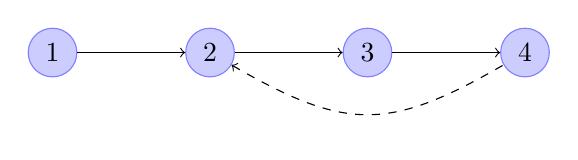
\begin{tikzpicture}[baseline=(s0.base)]
        % states
        \node[state] (s0) at (-2,2) {$1$};
        \node[state] (s1) at (0,2) {$2$}
            edge [<-] (s0);
        \node[state] (s2) at (2,2) {$3$}
            edge [<-] (s1);
        \node[state] (s3) at (4,2) {$4$}
            edge [<-] (s2);
        \draw [<-,dashed,bend right] (s1) to [looseness=1.25] (s3);
    \end{tikzpicture}
    }%
    \quad
    \subfloat[Modified prediction with loop removed.]{
    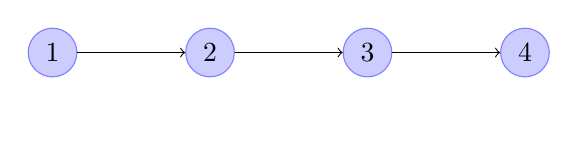
\begin{tikzpicture}[baseline=(s0.base)]
        % states
        \node[state] (s0) at (-2,2) {$1$};
        \node[state] (s1) at (0,2) {$2$}
            edge [<-] (s0);
        \node[state] (s2) at (2,2) {$3$}
            edge [<-] (s1);
        \node[state] (s3) at (4,2) {$4$}
            edge [<-] (s2);
        \draw [color=white,dashed,bend right] (s1) to [looseness=1.25] (s3);            
    \end{tikzpicture}
    }
    
    \caption{Example of heuristically removing loops. The nodes are numbered by the POI, with edges denoting order in the sequence. While the modified prediction removes the loop in the original sequence, it is necessarily at the expense of returning a path with fewer number of POIs.}
    \label{fig:heuristic}
\end{figure*}

